\documentclass[12pt]{article}
\usepackage[english]{babel}
\usepackage{color,soul}
\usepackage{apacite} 
\bibliographystyle{apacite}
\usepackage{url}
\usepackage[utf8x]{inputenc}
\usepackage{amsmath}
\usepackage[bottom]{footmisc}
\usepackage{graphicx}
\usepackage{pdfpages}
\graphicspath{{images/}}
\usepackage{parskip}
\usepackage{fancyhdr}
\usepackage{csvsimple}
\usepackage{booktabs}
\usepackage{longtable}
\usepackage{multirow}
\usepackage[title,titletoc,toc]{appendix}
\usepackage{vmargin}
\usepackage{listings}
\usepackage{pgfplotstable,filecontents}
\usepackage{natbib}
\usepackage{subfigure}
\usepackage{graphicx}
\usepackage{sidecap}
\usepackage{floatrow}
\usepackage[T1]{fontenc}
\usepackage{babel}
\usepackage[font=small,labelfont=bf]{caption}
\newfloatcommand{capbtabbox}{table}[][\FBwidth]
\usepackage{blindtext}
\usepackage{csvsimple}
\setlength{\bibsep}{5.0pt}
\pgfplotsset{compat=1.9}% supress warning
\setmarginsrb{2.5cm}{1.5cm}{2.5 cm}{1.5 cm}{1.5 cm}{1 cm}{1 cm}{1.5 cm}
\usepackage{color}

\definecolor{dkgreen}{rgb}{0,0.6,0}
\definecolor{gray}{rgb}{0.5,0.5,0.5}
\definecolor{mauve}{rgb}{0.58,0,0.82}
\definecolor{black}{rgb}{0,0,0}
\definecolor{white}{rgb}{1,1,1}
\definecolor{blue}{rgb}{0,0,1}
\lstset{ 
  language=R,                         
  basicstyle=\scriptsize,       
  numbers=left,                   		% where to put the line-numbers
  numberstyle=\tiny\color{gray},  	% the style that is used for the line-numbers
  stepnumber=1,                   		% the step between two line-numbers. If it's 1, each line will be numbered
  numbersep=5pt,                  		% how far the line-numbers are from the code
  backgroundcolor=\color{white},  	% choose the background color. must add \usepackage{color}
  showspaces=false,               		% show spaces adding particular underscores
  showstringspaces=false,        		 % underline spaces within strings
  showtabs=false,                		 % show tabs within strings adding particular underscores
  frame=single,                  			 % adds a frame around the code
  rulecolor=\color{black},       		 % if not set, the frame-color may be changed on line-breaks within not-black text (e.g. commens (green here))
  tabsize=2,                      			% sets default tabsize to 2 spaces
  captionpos=b,                   		% sets the caption-position to bottom
  breaklines=true,               		 % sets automatic line breaking
  breakatwhitespace=false,       		 % sets if automatic breaks should only happen at whitespace
  title=\lstname,                 			% show the filename of files included with \lstinputlisting;
                                 				 % also try caption instead of title
  keywordstyle=\color{blue},      		% keyword style
  commentstyle=\color{dkgreen},  	 % comment style
  stringstyle=\color{mauve},      		% string literal style
  escapeinside={\%*}{*)},         		% if you want to add a comment within your code
  morekeywords={*,...}           		 % if you want to add more keywords to the set
} 

\newtheorem{esti}{Theorem}[section]
\title{Modelling Fuel Economy Using Regression Analysis}					% Title
% * <akankshita.dash@u.nus.edu> 2016-11-08T05:26:27.242Z:
%
% ^.
\author{ST2137}							% Author
\date{08 November 2016}							% Date

\makeatletter
\let\thetitle\@title
\let\theauthor\@author
\let\thedate\@date
\makeatother

\pagestyle{fancy}
\fancyhf{}
\rhead{\theauthor}
\lhead{\thetitle}
\cfoot{\thepage}
\usepackage{setspace}
\begin{document}
\doublespacing
%%%%%%%%%%%%%%%%%%%%%%%%%%%%%%%%%%%%%%%%%%%%%%%%%%%%%%%%%%%%%%%%%%%%%%%%%%%%%%%%%%%%%%%%%


%%%%%%%%%%%%%%%%%%%%%%%%%%%%%%%%%%%%%%%%%%%%%%%%%%%%%%%%%%%%%%%%%%%%%%%%%%%%%%%%%%%%%%%%%

\begin{titlepage}
	\centering
    
\includegraphics[width = 0.4\textwidth]{logo1.jpg}\\[0.4cm]	% University Logo
    \textsc{ National University of Singapore}\\[0.2 cm]	% University Name
	\rule{\linewidth}{0.2 mm} \\[0.1 cm]
	{ \huge \bfseries \thetitle}\\
	\rule{\linewidth}{0.2 mm} \\[0.2 cm]
	
\section*{Executive Summary}
This report serves to find the factors that contribute to the fuel economy of a car. Small cars were found to be the most fuel efficient, while types of cars were found to be highly correlated to weight. Weight was found to be the major factor that contributes to the variance of fuel economy. 	
	 
			\begin{center} 
			\textbf { ST2137 Computer Aided Data Analysis\\SEM 1, AY2016/2017}\\[0.7cm]
			\emph{Submitted By :}\\[0.1cm]
        Akankshita Dash (A0132788U), Drishti Baid (A0119586R), Jerome Cheang Yue Liang (A0114154U), Nelson Tan (A0124473J), Rowena Mairi Piers (A0152905H), Shabbeer Ahmad (A0140252X)\\[0.1cm] 
		    \end{center}
        


\end{titlepage}

%%%%%%%%%%%%%%%%%%%%%%%%%%%%%%%%%%%%%%%%%%%%%%%%%%%%%%%%%%%%%%%%%%%%%%%%%%%%%%%%%%%%%%%%%




%%%%%%%%%%%%%%%%%%%%%%%%%%%%%%%%%%%%%%%%%%%%%%%%%%%%%%%%%%%%%%%%%%%%%%%%%%%%%%%%%%%%%%%%%
\section{Problem Description}
Vehicles have played a vital role in our economy by facilitating transport and trade across distant places. To keep up with these developments, the number of cars has increased which results in a huge consumption of our limited fuel resources and damages our environment. Transportation takes up to half of the world’s oil resources and the number of cars will be tripled by the end of 2050 with most of them coming from emerging economies (\cite{FIA}). 

To support the increasing energy demand due to transportation, improvements on energy efficiency are required to curb the negative global impacts. Fuel economy, a measure of energy efficiency in automobiles, can play a vital role in reducing energy consumption and emissions of greenhouse gases. Fuel economy determines how far a vehicle can run on a gallon of fuel, which is commonly known as mileage per gallon (MPG). There are many factors that fuel economy depends on, hence it is important to understand how several defining factors can affect fuel economy. This will be useful to individuals, manufacturers and governments.  

In this report, our team will be analyzing different factors that will influence fuel economy and provide insights based on our results. 


%%%%%%%%%%%%%%%%%%%%%%%%%%%%%%%%%%%%%%%%%%%%%%%%%%%%%%%%%%%%%%%%%%%%%%%%%%%%%%%%%%%%%%%%%
\section{Data Description}
\subsection{Dataset}
 

\textbf{Type Of Car:} This is a categorical variable that includes small, sporty, compact, midsize and large cars. \newline
 \textbf{City MPG (Miles Per Gallon In The City):} City MPG is calculated by the total number of miles travelled in the city per gallon of fuel. This data was provided by EPA fuel efficiency ratings. City MPG will represent fuel economy and is the dependent variable.\newline
\textbf{Weight:} Weight of the car in pounds.\newline
\textbf{Revolutions per Minute (RPM):} Revolutions per minute at maximum horsepower.\newline
\textbf{Maximum Horsepower:} Power of the engine. \newline  
\textbf{Domestic:} Dummy which is = 0 if car is from a non-US manufacturer, and = 1 if car is from a US manufacturer.          

\section{Section I: Finding the Most Fuel Efficient Car}
\subsection{Discussion Of Statistical Analysis}
R is used to find the means of City MPG for each type of car. A box-plot is created to provide an overview of how each type of car performs. One way ANOVA is conducted to check if there are significant differences in the mean and the contrast method was used to establish how different the means are for each type of car. Finally, we proceed to check the assumptions of equal variance and normality. Since ANOVA is fairly robust, equal variance assumptions were relaxed.

%%%%%%%%%%%%%%%%%%%%%%%%%%%%%%%%%%%%%%%%%%%%%%%%%%%%%%%%%%%%%%%%%%%%%%%%%%%%%%%%%%%%%%%%%%%%%%%%%%%%%%%%%%%%%%%%%%%%%%%%%%%%%%%%%%%%%%%%%%%%%%%%%%%%%%%%%%%%%%%%%%%%%%%%%%%%%%%%%%
\subsection{Interpretation of Findings}
\begin{figure}[!htb]
	\caption*{\textbf{Fig I}: Boxplot of City MPG and Type Of Car}
	\begin{center}
	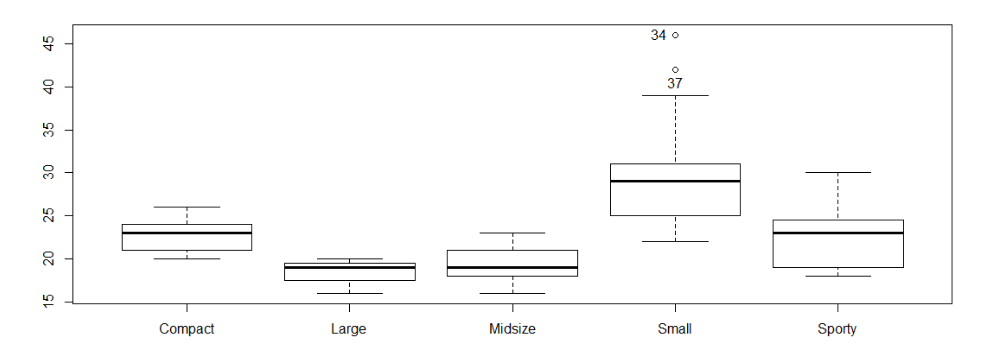
\includegraphics[width=0.80\textwidth]{Boxplot.png}
	\end{center}
\end{figure}

Fig I shows that small cars are the most fuel efficient with a City MPG mean of 29.85714 while the least fuel efficient are large vehicle with a City MPG mean of 18.36364. By using contrast method, there was insignificant evidence to show that there is a mean difference when we compare the means of "Large vs Midsize". However, significant mean differences can be observed when we compare means of "Sporty vs Large and Midsize", "Compact vs Large, Midsize,and Sporty" and "Small vs Large, Compact, Midsize, and Sporty".

We also interpret that there may be some relationship between weight and City MPG as the means of City MPG decreases when transitioning from lighter cars to heavier vehicles occurs. Based on the interpretation of results, weight becomes an important factor to consider when maximizing fuel efficiency. As heavier cars have higher inertia and greater rolling resistance, they require more energy to move thus more fuel is being consumed (\cite{NRC}). In the next part, we will conduct exploratory analysis on weight and perform linear regression model analysis.
%%%%%%%%%%%%%%%%%%%%%%%%%%%%%%%%%%%%%%%%%%%%%%%%%%%%%%%%%%%%%%%%%%%%%%%%%%%%%%%%%%%%%%%%%
%%%%%%%%%%%%%%%%%%%%%%%%%%%%%%%%%%%%%%%%%%%%%%%%%%%%%%%%%%%%
\section{Section II: Analyzing Weight and Fuel Economy}
\textbf{Stage 1}: Checking for a linear relation between weight and fuel economy \newline
\textbf{Scatter plot}: We begin the analysis by plotting a scatter plot between CityMPG and the weight of a car.
\begin{figure}[!htb]
	\begin{center}	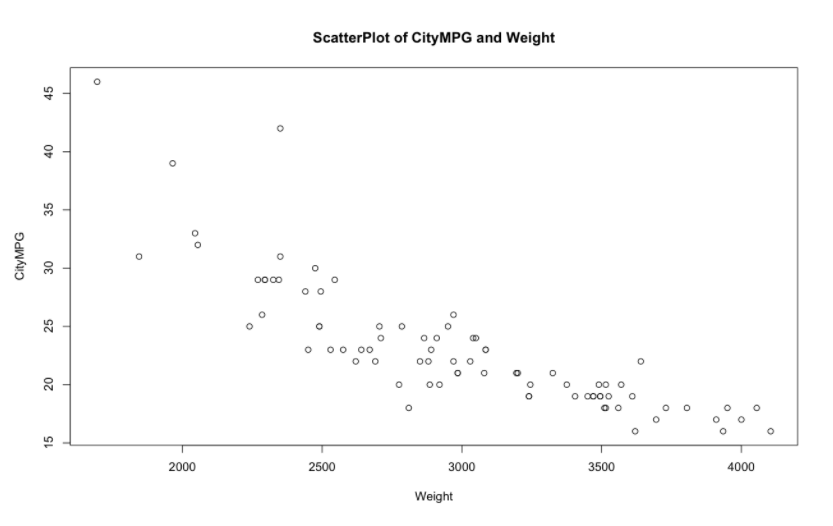
\includegraphics[width=0.60\textwidth]{Scatterplot.png}
    \caption*{\textbf{Fig II}:{ Scatterplot Of CityMPG and Weight}}
	\end{center}
\end{figure}
We first compute the correlation coefficients from the sample: 
\lstinputlisting[firstline=1, lastline=9]{Results.R}
From the results we see that there is a strong negative correlation of -0.83 between weight and fuel economy. 
\subsection{Developing Regression Models}
We developed 4 methods to build our model: 
\begin{itemize}
\item \textbf{Simple Linear Regression on CityMPG and Weight}

\item \textbf{Transformation on Linear Regression}

\item \textbf{Multiple Regression of CityMPG with Weight + Type}

\item \textbf{Multiple Regression of City MPG with other variables}
\end{itemize}
\textbf{Model 1: Simple Linear Regression} \newline
Coefficient of Determination (R-Square) is 0.69, which means that weight of cars explains 69\% of variation in fuel efficiency.

\begin{figure}[!htb]
	\caption*{\textbf{Fig III }:{QQPlot and Residual Plot Of City MPG and Weight}}
	\begin{center}
	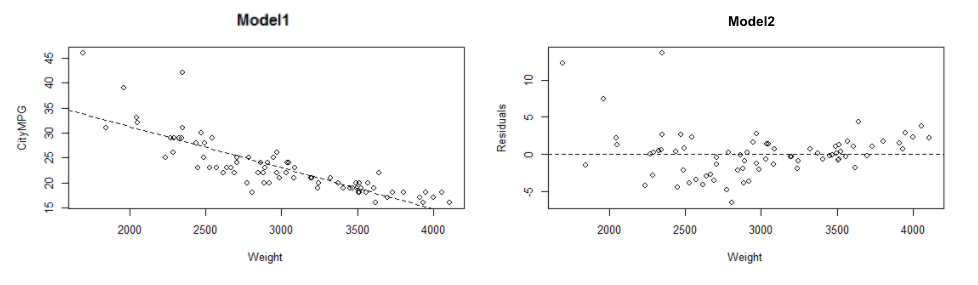
\includegraphics[width=0.8\textwidth]{Residual.png}
	\end{center}
\end{figure}

From Fig III, there seems to be a decreasing function in the linearity graph and a U shape in the  residual plots. 
We apply transformation to the model and come up with two models - one with quadratic terms and another with an inverse transformation.


\textbf{Model 2: Transformed Linear Regression} \newline
From Fig III, we see that there is a decreasing relation. 


We compared the following models: \newline
2a) CityMPG = $\beta_0 + \beta_1(Weight) + \beta_2(Weight^{2})$ \newline
2b) CityMPG = $\beta_0 + \beta_1(\frac{1}{Weight})$ 


Comparing the models, we chose model2b as it has fewer variables and a better adjusted R-square of 0.7767.


\textbf{Model 3: Multiple Regression of CityMPG with Weight + Type} 
\begin{figure}[!htb]
	\begin{center}
	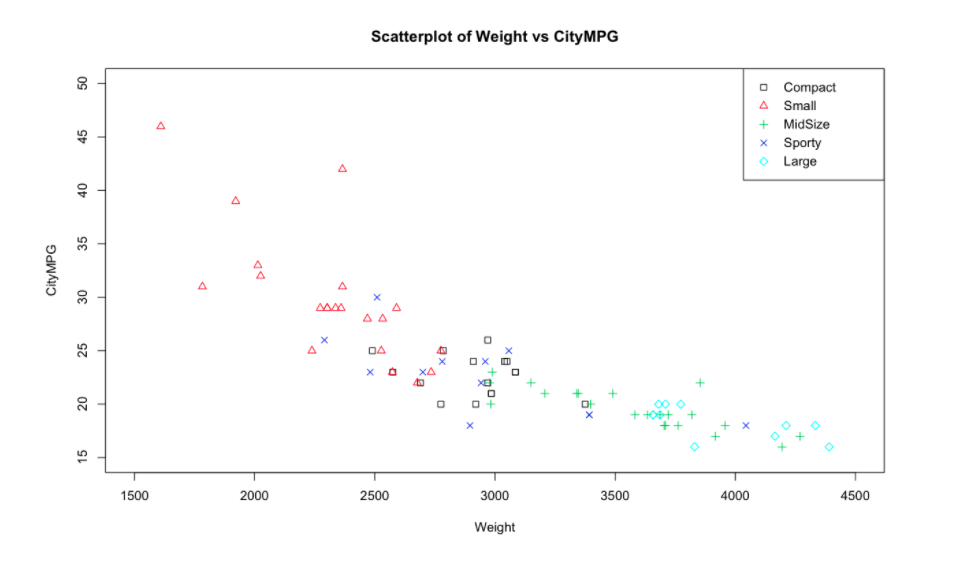
\includegraphics[width=0.6\textwidth]{ScatterplotType.png}
    \caption*{\textbf{Fig IV}:{ Scatterplot Of CityMPG and Weight classified by Type}}
	\end{center}
\end{figure}\newline
From Fig IV, the types were clustered together along the x-axis, showing that there is a strong correlation between Type and Weight. We intend to model the following variables to check for \textbf{Omitted Variable Bias}. However, the adjusted R$^{2}$ dropped from 0.7767 to 0.7753.  It means that weight have a higher explanatory power compared to Type, thus Type is dropped from the model to reduce multicollinearity. 



\textbf{Model 4: Inclusion of other explanatory variables } \newline
\begin{figure}[!htb]
	\caption*{\textbf{Fig V}:{ QQPlot and Residual Plot Of City MPG and Weight}}
	\begin{center}
	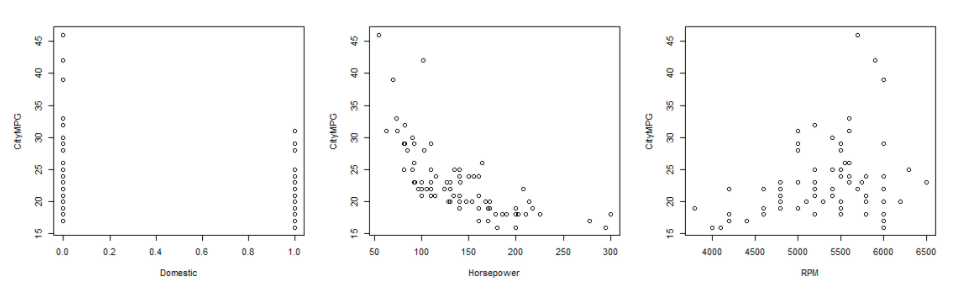
\includegraphics[width=0.9\textwidth]{Other_variables.png}
	\end{center}
\end{figure}

We look to incorporate other variables may have some explanation of fuel efficiency variance. 
Some examples are Domestic, Horsepower and RPM. Scatterplots of the independent variable were plotted against fuel efficiency and transformation was done to the variables if they are less likely to have a linear relationship(Fig V).

From our findings, we see that there is only a slight increase in the adjusted R-square in the model when we add Domestic as a variable (0.003), while the other 2 variables (horsepower and RPM) result in decreased adjusted R-square. Even though there is a slight increase in adjusted R-square, the p-value of Coefficient for Domestic shows that it is not significant. 

\subsection{Interpretation of findings}
We chose model 2b as it provided the best R-square and fewest variables. The model can be interpreted as follows: 
\begin{center}
$CityMPG = -0.8901+ 68959(\frac{1}{Weight}) + \epsilon$
\end{center}
As the weight increases, CityMPG decreases. Using mean weight of 2988.171, if we increase weight by 10\%, CityMPG will decrease by 9.45\%. 
We conclude that weight contributes to the most variance in fuel efficiency. 
\subsubsection{Assumption testing}

\begin{figure}[!htb]
	\caption*{\textbf{Fig VI }:{QQPlot and Residual Plot Of City MPG and Weight}}
	\begin{center}
	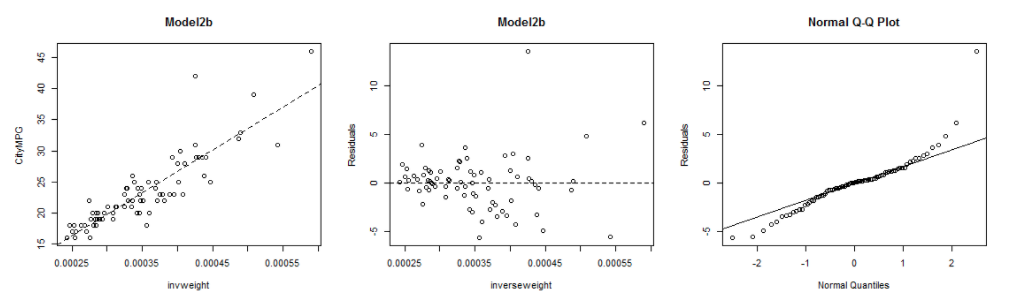
\includegraphics[width=0.8\textwidth]{Assumption.png}
	\end{center}
\end{figure}

Linear Regression has linearity assumptions, equal variance and normality assumptions.From Fig VI, it seems that there is linearity across City MPG and invweight. Residuals plot shows equal spread of variance across the plots. Normality plot shows a slight tail at the end of the normal quantile. However, using One-sample Kolmogorov-Smirnov test, there is insignificant evidence that the residuals from the model are not normal. 
\subsubsection{Limitations}
We acknowledge that there are some limitations to our usage of data as the data pool is small and outdated, which may not be a suitable representation of the car population in fuel economy. However, a 2016 report suggests that weight is one of the factors that has a trade-off with fuel economy in the Spanish car market. (\cite{IEB}). This can also be generalized to cover the world car market - which means that our interpretation is still relevant even with these current limitations in the data. 
%%%%%%%%%%%%%%%%%%%%%%%%%%%%%%%%%%%%%%%%%%%%%%%%%%%%%%%%%%%%%
\section{Conclusion}
From Section I, we conclude that there is significant evidence that small cars are the most fuel efficient. 
From Section II, we conclude that weight and fuel efficiency have an inverse relation. The regression model suggests that weight explains about 77\% of the variation in the fuel economy of a car and thus weight is a crucial Passdeterminant of City MPG. Weight is an important factor to consider when maximising fuel efficiency. These results correspond with trends found in the United States automobile industry, demonstrated by the relationship between car weight and fuel economy (\cite{IWU}).



%%%%%%%%%%%%%%%%%%%%%%%%%%%%%%%%%%%%%%%%%%%%%%%%%%%%%%%%
Overall, this report adopts rigorous statistical regression analysis based on reliable data as well as critical reasoning based on secondary research, both of which the team reckons has manifested the meaningfulness and importance of this project.
\newpage
\bibliography{biblio.bib}
\begin{appendices}
%%%%%%%%%%%%%%%%%%%%%%%%%%%%%%%%%
%%%%%%%%%%%%%%%%%%%%%%%%%%%%%%%%%
%%%%%%%%%%%%%%%%%%%%%%%%%%%%%%%%%%
\section{Clean Data Sheet} \label{app:CLData}
\csvautobooklongtable[respect sharp]{Cars.csv}\label{Tab:CLData}
%%%%%%%%%%%%%%%%%%%%%%%%%%%%%%%%%%
\section{Main Code For Part 1 Analysis} \label{app:Part1Code}
\lstinputlisting{Part1.txt}
%%%%%%%%%%%%%%%%%%%%%%%%%%%%%%%%%%%
%%%%%%%%%%%%%%%%%%%%%%%%%%%%%%%%%%
%%%%%%%%%%%%%%%%%%%%%%%%%%%%%%%%%%
\break
\break 
\break
\section{Main Code For Part 2 Analysis} \label{app:Part2Code}
\lstinputlisting{Part2.txt}
%%%%%%%%%%%%%%%%%%%%%%%%%%%%%%%%%%%
\end{appendices}
\end{document}